%%%%%%%%%%%%%%%%%%%%%%%%%%%%%%%%%%%%%%%%%%%%%%
%                insertmeeting
% 1) Title (something creative & funny?)
% 2) Date (MM/DD/YYYY)
% 3) Location (ex. Hagerty High School)
% 4) People/Committees Present 
% 5) Picture 
% 6) Start Time & Stop Time (ex. 12:30AM to 4:30PM)
%%%%%%%%%%%%%%%%%%%%%%%%%%%%%%%%%%%%%%%%%%%%%%
\insertmeeting 
	{Meeting Example} 
	{11/27/21}
	{Hagerty High School}
	{Clayton, Nathan, Ritam}
	{Images/RobotPics/robot.jpg}
	{2:30 - 4:30}
	
\hhscommittee{Hardware}
\noindent\hfil\rule{\textwidth}{.4pt}\hfil
\subsubsection*{Goals}
\begin{itemize}
    \item Add flanges to carbon fiber side CAD
    \item Create molds for carbon fiber sides in CAD
 

\end{itemize} 

\noindent\hfil\rule{\textwidth}{.4pt}\hfil

\subsubsection*{Accomplishments}
Continuing our work from yesterday, we started creating the molds for the carbon fiber sides. These are the important parts, as they are what will actually be printed and used to create the side plates. Not having a real idea of how we would create the molds based on the sides we made in Onshape at the last meeting, we started looking for ways that we could easily create the mold. We soon found out about the thicken tool, which works perfectly for what we need. By selecting each face of the sides, we were able to create the molds to fit perfectly against the sides (Figure \ref{fig:pic1}). After creating the base of the molds, we thought of one more feature that we wanted to add to the sides to make them stronger.  Although carbon fiber is already very strong, a thin plate of it can still be flexible. To counteract the thinness of the plate, we wanted to add flanges to the outside of the sides, which will essentially add depth to the sides without taking up much more space or weight. Adding the flanges was a simple process of creating sketches on each end of the carbon fiber sides and extruding (Figure \ref{fig:pic2}). 
With the final changes made to the side plates, we added the flanges onto the mold and started thinking about how the part would print. Because of the weird shape of the sides, simply printing them upright would be unstable and might use more support material than necessary. Looking at the mold from the side, we noticed that the most efficient way to  print the model would be at a slight angle to minimize the amount of support material needed (Figure \ref{fig:pic3}). We planned to extend the mold out to this line, then create our own supports in a grid pattern. This is needed so that when we form the carbon fiber over the mold and press it down with the vacuum pump, the mold will stay supported in the right position. Without the supports,not only would it take longer to print, but we would face the risk of the mold tipping while the carbon fiber is formed over it. To make these supports, we created a planeat the angle shown in figure 3 and sketched a grid. We added more lines to the grid at the lowest points of the mold to ensure every point was well supported (Figure \ref{fig:pic4}). Because the 2 sides are different from each other, we had to repeat this process to finish both molds (Figure \ref{fig:pic5}). Once we print these molds, we will be able to start making the sides out of carbon fiber.

 

\begin{figure}[ht]
\centering
\begin{minipage}[b]{.48\textwidth}
  \centering
  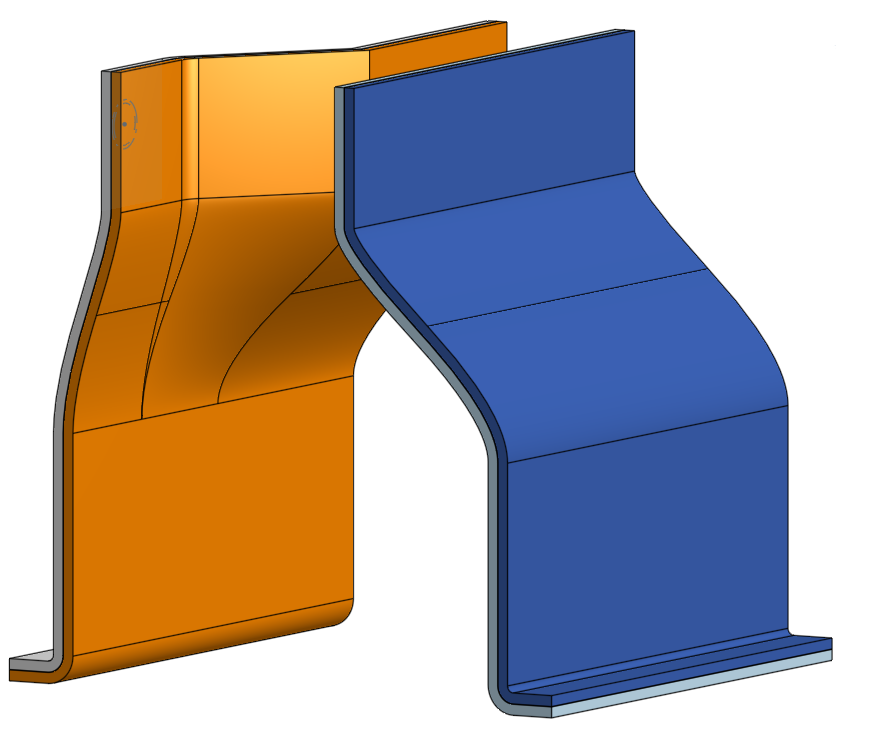
\includegraphics[width=0.95\textwidth]{Meetings/November/11-27-21/11-22-21_CAD_Figure1 - Nathan Forrer.PNG}
  \caption{Molds for both sides}
  \label{fig:pic1}
\end{minipage}%
\hfill%
\begin{minipage}[b]{.48\textwidth}
  \centering
  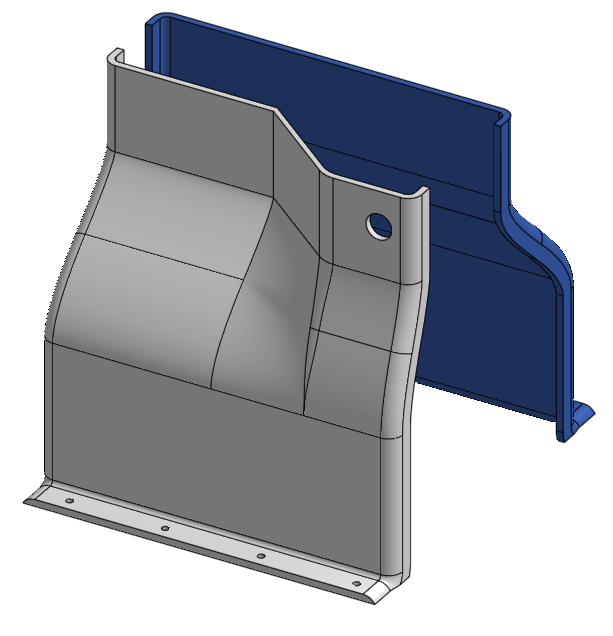
\includegraphics[width=0.95\textwidth]{Meetings/November/11-27-21/11-22-21_CAD_Figure2 - Nathan Forrer.PNG}
  \caption{Adding flanges to the sideplates}
  \label{fig:pic2}
\end{minipage}
\end{figure}

\begin{figure}[ht]
\centering
\begin{minipage}[b]{.48\textwidth}
  \centering
  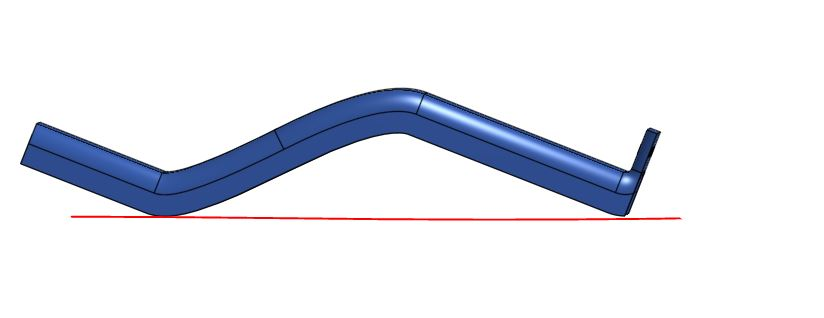
\includegraphics[width=0.95\textwidth]{Meetings/November/11-27-21/11-27-21_CAD_Figure3 - Nathan Forrer.JPG}
  \caption{Printing at a slight angle to maximize efficiency}
  \label{fig:pic3}
\end{minipage}%
\hfill%
\begin{minipage}[b]{.48\textwidth}
  \centering
  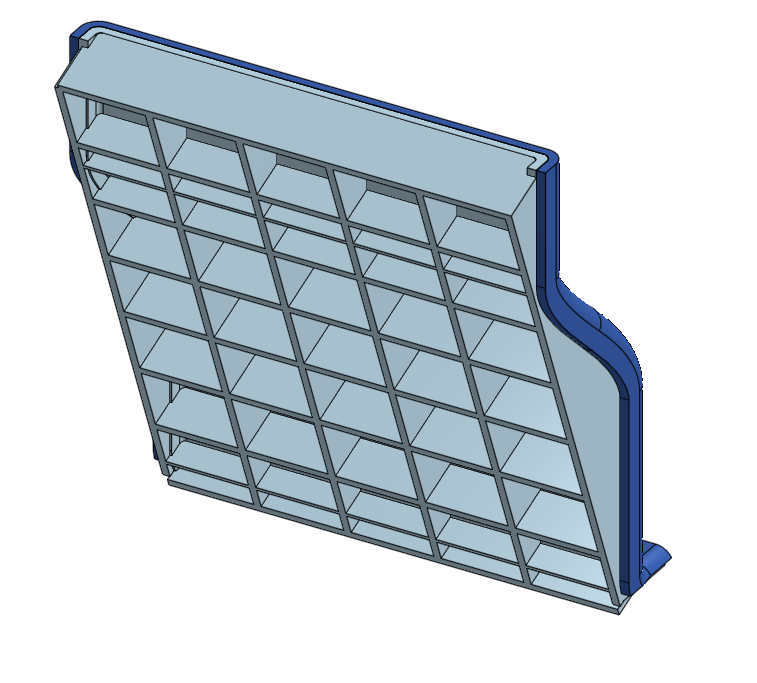
\includegraphics[width=0.95\textwidth]{Meetings/November/11-27-21/11-22-21_CAD_Figure4 - Nathan Forrer.PNG}
  \caption{The supports created during printing}
  \label{fig:pic4}
\end{minipage}
\end{figure}

\begin{figure}[htp]
\centering
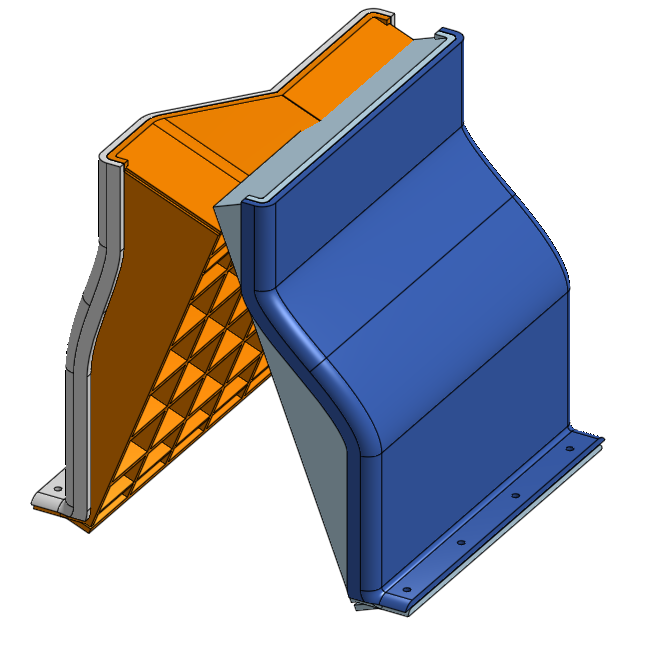
\includegraphics[width=0.95\textwidth, angle=0]{Meetings/November/11-27-21/11-22-21_CAD_Figure5 - Nathan Forrer.PNG}
\caption{The ready-to-print molds}
\label{fig:pic5}
\end{figure}



\whatsnext{
\begin{itemize}
    \item 3d print carbon fiber side molds
    \item Use mold to create sides out of carbon fiber 

\end{itemize} 
}

